\section{Our Approach}

Before we discuss our approach for splitting TV watching sequence, we give some definitions and heuristics first.

\emph{Definition 1:} $Prob(S|P_1,P_2)$ is the probability that program $P_1$ and program $P_2$ viewed by the same viewer.

\emph{Definition 2:} Bi-gram Program Pair refers to any two adjacent programs in the viewing sequence.

\emph{Definition 3:} Time Continuity Group refers to a sub-sequence of the viewing sequence such as for any bi-gram program pairs from this sub-sequence the end time of the first program is equal to the start time of the second program.

\emph{Heuristic 1:}If tow programs are watched continuously, then they are likely be watched by a single viewer.

\emph{Heuristic 2:}If two programs are watched continuously and the switching time is the start time of the second
 program, then they are most probably watched by a single viewer. An illustration is depicted in figure \ref{fig:2}

\begin{figure}[htbp]
\centering
\includegraphics[width=2.5in]{h2.eps}
\caption{Illustration of Heuristic 2}
\label{fig:2}
\end{figure}

\subsection{Mining Prior Knowledge}
According to Heuristic 1 and Heuristic 2, we could mine some prior knowledge from given viewing sequences.
The first knowledge leant from given viewing sequences is $Prob(S|P_1,P_2)$ if $P_1$ and $P_2$ are viewed continuously.
The second knowledge leant from given viewing sequences is $Prob(S|P_1,P_2)$ if $P_1$ and $P_2$ are viewed continuously and
the start time of program $P_2$ is between the threshold and switching time. The algorithm for mining these two knowledge is
depicted in algorithm \ref{code:2}.

\begin{algorithm}[htb]
\caption{Mining Prior Knowledge}
\label{code:2}
\begin{algorithmic}[1]
\STATE $bigramCount = 0$
\STATE $h1Count=0$
\STATE $h2Count=0$
\STATE $index=0$
\WHILE{$index < prog.size()-1$}
\STATE $first=prog.get(index)$
\STATE $second = prog.get(index+1)$
\STATE $inc(bigramCount);inc(index)$
\IF{$CHECKH1(first,second) == true$}
\STATE $inc(h1Count)$
\IF{$CHECKH2(first,second) == true$}
\STATE $inc(h2Count)$
\ENDIF
\ENDIF
\ENDWHILE
\end{algorithmic}
\end{algorithm}

Usually, the collected viewing sequences are unlabeled. Thus, before the mining prior knowledge algorithm processing, we need
first select some sequences and label them as the training set. After we generate a training set, we could carry out the mining
algorithm and get two prior probabilities. The mining task could be repeated for different training set and different time.
Averaged result could be treated as prior knowledge.

\subsection{Markov Chain Model}
By using prior knowledge, we've already got some useful information to help us finish the splitting task.
However, we find the bi-gram program pair which could be used for generating prior knowledge is very few.
Yet, we notice that some programs are viewed continuously. For example, program $P_1$,$P_2$,$P_3$ are continuous
to each other. From mining prior knowledge algorithm, bi-gram program pairs $<$$P_1$,$P_2$$>$ and $<$$P_2$,$P_3$$>$ are
assigned probability value to help the splitting task. However, by our common sense, we know the program pair
$<$$P_1$,$P_3$$>$ would also be useful because these two programs are sticked by time continuity. In order to mining
probability like $Prob(S|P_1,P_3)$, we came up with a Markov chain model\cite{1003838}\cite{18626}\cite{1165342}\cite{Baier:2003:MAC:1435631.859038}.

There is a type of random process which could be characterized as memory-less. We call such random process Markov process.
And if the state set is finite we call the Markov process Markov chain.

If the state of random variable X forms a Markov chain, then $P{(X_{n+1}=j|X_n=i)}$ expresses the probability at time $n$ X
is in state i and the next state of i is j. Usually the next state only depends on the current state regardless of time $n$.
Then we could express the probability of state transition as a matrix.

\begin{equation}
\boldsymbol{P}=(p_{ij})=
\begin{bmatrix}
p_{00} & p_{01} & p_{02} & \cdots \\
p_{10} & p_{11} & p_{12} & \cdots \\
p_{20} & p_{21} & p_{22} & \cdots \\
\vdots & \vdots & \vdots &
\end{bmatrix}
\end{equation}

$p_{ij}^{(n)}=P{(X_{m+n}=j|X_m=i)}$ expresses the probability the next state of i is j after n step. Here n step means
repeating the strategy n times.
Then given the initial probability distribution of all objects involved in the strategy, we could find the probability of our
interested object.

From mining prior knowledge algorithm, we could know the probability $Prob(S|P_1, P_2)$ if $P_1$ and $P_2$ are continuous
in time. There are two possible values for $Prob(S|P_1, P_2)$:

\begin{equation}
\left\{
\begin{aligned}
\begin{array}{cc}
Prob(S|P_1, P_2)&=\alpha\ if\ p_1\ and\ p_2\ satisfy\ heuristic\ 1 \\
Prob(S|P_1, P_2)&=\beta\ if\ p_1\ and\ p_2\ satisfy\ heuristic\ 2
\end{array}
\end{aligned}
\right.
\end{equation}

In our method, we use prior knowledge $\alpha$ and $\beta$ to calculate $Prob(S|P_1, P_2)$ if $P_1$ and $P_2$ have time continuity
relation between each other but aren't adjacent to each other. That is, we have $N$ programs in the viewing sequence
$P_1,P_2,P_3,\cdots,P_n$ and $P_i$ and $P_{i+1}$($1 \leq i \leq n-1$) are bi-gram program pair. We use Markov chain model to calculate
$Prob(S|P_i,P_j)$($i \le j \leq n$)

We first build the transition matrix of the Markov chain. The matrix is depicted blow. There are two characteristics of the transition
matrix. First, according to Markov chain theory, the sum of all probabilities in a row is equal to 1. Secondly, for row $i$, expect for
$Prob(S|P_i,P_i)$ and $Prob(P_i, P_{i+1})$, other probabilities are all zero for we only know the probability of two continuous programs.

\begin{equation}
\boldsymbol{P}=(p_{ij})=
\begin{bmatrix}
1-\alpha & \alpha  & 0 & 0 &  \cdots & 0 & 0 \\
0 & 1-\beta & \beta & 0 & \cdots & 0 & 0 \\
0 & 0 & 1-\beta & \beta & \cdots & 0 &0 \\
\vdots & \vdots & \vdots & \vdots & \cdots & \vdots & \vdots \\
0 & 0 & 0 & 0 & \cdots & 1-\alpha & \alpha \\
0 & 0 & 0 & 0 & \cdots & 0 & 1
\end{bmatrix}
\end{equation}

After we have built transition matrix, we could compute $Prob(S|P_i,P_j)$ where program $P_i$ and $P_j$ are in the same time continuity
group and $i < j \leq n$. We give the formula for calculating $Prob(S|P_i,P_j)$ first and then explain it.

\begin{equation}
Prob(S|P_i, P_j) = V_i \times \boldsymbol{P}^{(j-i)}[j]
\end{equation}

Here $V_i$ stands for a vector whose $i$-th column is 1 and other column is 0. $\boldsymbol{P}^{(j-i)}$ stands for the $(j-i)$-step
transition matrix and $\boldsymbol{P}^{(j-i)}[j]$ stands for the $j$-th column of the $(j-i)$-step transition matrix.

$V_i$ stands for the initial probability distribution of n programs. We assume only the $i$-th program is being viewed now. After
$(j-i)$ times program switching, we could calculate the probability that the user is viewing the $j$-th program. So, according to
Markov chain theory, the probability the user at $j$-th program is $V_i \times \boldsymbol{P}^{(j-i)}[j]$. In other words, the
probability concluded from Markov chain theory is same as the probability that program $P_i$ and $P_j$ are viewed by same viewer,
namely $Prob(S|P_i,P_j)$.

Noticing the special form of transition matrix, we could simplify the calculation for $Prob(S|P_i,P_j)$. Suppose there are k programs
viewed between $P_i$ and $P_j$($k=j-i-1$).Then the formulation could be simplified as follows:

\begin{equation}
Prob(S|P_i,P_j)=\prod_{k=i}^{j-1}Prob(S|P_k,P_{k+1})
\end{equation}

$Prob(S|P_k,P_{k+1})$ has already given by mining prior knowledge algorithm. Thus we could calculate probability between $P_i$ and
$P_j$ if $P_i$ and $P_j$ are in the same time continuity group and $i<j$.

By utilizing Markov chain theory, we expand prior probability to more programs. The simplified formula could give us the probability
between two programs in a time continuity group efficiently. Meanwhile, Markov chain theory tells us this probability is reliable.
In the following sub-section, we will use the probability which has concluded now to split viewing sequence.

\subsection{Attribute Co-occur Matrix}
By using prior knowledge and Markov chain model, we could find $Prob(S|P_1,P_2)$ if program $P_1$ and $P_2$ are in the same time
continuity group. However, we are interested in $Prob(S|P_1,P_2)$ for each pair of program in the viewing sequence. In order to
calculate this probability between any two program, we first introduce the attribute co-occur
technique\cite{He:2006:ACS:1132863.1132872}\cite{4734002}\cite{4401042}.

The basic idea is that $Prob(S|P_1,P_2)$ could be used as the program attributes' similarity between these two programs. And if
we record all attributes' similarity from known $Prob(S|P_1,P_2)$ then this matrix could be used as another prior knowledge.

In our implementation, there're 6 attributes for each program. And for each program, the values for this attribute is obtained
from internet by an automatic extraction program. The extraction program will start in the previous weekend and according to
downloaded schedule extract values automatically.

For example, we have two attributes $A_1$ and $A_2$, and there are $N$ programs containing these two attributes. That is,
$P_1$,$P_2$,$\cdots$,$P_n$. Then we could express $Prob(A_1,A_2)$ as follows:

\begin{equation}
Prob{(A_1,A_2)}=\frac{\sum_{k=1}^{N-1}Prob(S|P_k,P_{k+1})}{N}
\end{equation}

We need two iteration to generate attribute co-occur matrix. The first iteration extracts all attribute value into a pre-defined
attribute list. The second iteration check all program pairs and if the two programs $P_1$ and $P_2$ have already been processed
in previous knowledge generation module update attribute value pairs from $P_1$ and $P_2$ with the probability $Prob(S|P_1,P_2)$.
The pseudo-code for building attribute co-occur matrix is in algorithm \ref{code:3}.

\begin{algorithm}[htb]
\caption{Building Attribute Co-Occur Matrix}
\label{code:3}
\begin{algorithmic}[1]
\STATE $attrList = NULL$
\STATE $attrCo[][] = NULL$
\STATE $attrCoCount[][] = NULL$
\FORALL{$prog \in progList$}
\FORALL{$value \in prog.attribute$}
\IF{$value \notin attrList$}
\STATE $attrList.add(value)$
\ENDIF
\ENDFOR
\ENDFOR
\WHILE{$index < progList.size-1$}
\STATE $first=progList.get(i)$
\STATE $second = progList.get(i+1)$
\FORALL{$value_1 \in first$}
\FORALL{$value_2 \in second$}
\STATE $attrCo[indexof(value_1)][indexof(value_2)] += Prob(S|first,second)$
\STATE $inc(attrCoCount[indexof(value_1)][indexof(value_2)])$
\ENDFOR
\ENDFOR
\STATE $inc(index)$
\ENDWHILE
\STATE $i=0;j=0$
\WHILE{$i < attrList.size$}
\WHILE{$j < attrList.size$}
\STATE $attrCo[i][j] /= attrCoCount[i][j]$
\STATE $inc(j)$
\ENDWHILE
\STATE $inc(i)$
\ENDWHILE
\end{algorithmic}
\end{algorithm}

Attribute co-occur matrix will serve as the final knowledge for the following splitting task. There are two main benefits of using
attribute co-occur matrix. The first one is attribute co-occur matrix not only concludes the knowledge we have mined but also expand
it to a more expressive and meaningful format. The second one is attribute co-occur matrix are easy to understand both for researchers
and for machines.

And there are some alternatives for the range of attribute. The first one is the attribute comes from the sequence considered. And the
second one is attribute comes from several sequences. If we use the second one, then we could combine more knowledge together. And if
the user behind these sequences are same, then this combination would great benefit the splitting result.

In the next sub-section, we will introduction how to use attribute co-occur matrix to build $P(S|P_1,P_2)$ for each pair of program in the
viewing sequence.

\subsection{Probability Model}
By using attribute co-occur matrix, we could find $Prob(S|P_1,P_2)$ for any two programs in the sequence. We first give the formula for
calculating $Prob(S|P_1,P_2)$:

\begin{equation}
Prob(S|P_1,P_2)=\frac{\sum_{a_1 \in P_1, a_2 \in P_2}{Prob(S|a_1, a_2)}}{||P_1||\times||P_2||}
\label{eq:1}
\end{equation}

Here, $||P_i||$ stands for the size of attributes for program $P_i$. And from statistics perspective, equation \ref{eq:1} is the mean
of prior knowledge probability for all attribute pairs involved in program $P_1$ and $P_2$.

It's easy to understand this definition. The probability the user watches $P_1$ and $P_2$ is determined by the probability of attribute pairs from these
two programs. And notice that $Prob(S|a_1,a_2)$ is the probability that $a_1$ and $a_2$ is viewed by a single viewer. So $Prob(S|P_1,P_2)$ likes a voting
result from all attribute pairs.

And if we use alternative 2 to calculate attribute co-occur matrix, then we could get $Prob(S|a_1,a_2)$ from a global perspective. Thus the voting result
$Prob(S|P_1,P_2)$ will be more accurate. The pseudo-code for calculating the $Prob(S|P_1,P_2)$ is in algorithm \ref{algo:4}.

\begin{algorithm}[htb]
\caption{Calculate Probability for Each Program Pair}
\label{algo:4}
\begin{algorithmic}[1]
\STATE $prob[][] = double[progSize][progSize]$
\FORALL{$prog_1 \in progs$}
\FORALL{$prog_2 \in progs$}
\STATE $AttrCount=0$
\STATE $sum = 0$
\FORALL{$a_1 \in prog_1$}
\FORALL{$a_2 \in prog_2$}
\STATE $inc(AttrCount)$
\STATE $sum += Prob(a_1,a_2)$
\ENDFOR
\ENDFOR
\STATE $prob[indexof(prog_1)][indexof(prog_2)]=sum/AttrCount$
\ENDFOR
\ENDFOR
\end{algorithmic}
\end{algorithm}

By using voting methods to calculate $Prob(S|P_1,P_2)$, we could avoid the problems discussed in baseline algorithm. For example, if a user watches both sports program
and news program, then in our baseline algorithm, we could never find similarity between these two programs. However, in our approach, the algorithm could first find
some prior knowledge from the viewing sequences which connects sports program and news program and then give us an accurate similarity score for these two programs.
And consider another case where both two users like sports program. In our baseline approach, two sports programs will be assigned a high similarity score but they
are not watched by a same viewer. And in our approach, these two programs may be assigned a low probability because we could not find supporting knowledge for these
two program. So our approach solve the problem that users may have multi-interests.

\subsection{Clustering}
We could use the generated probability $Prob(S|P_1,P_2)$ of each program pair as the input to the clustering algorithm to generate a set of program sub-sequences.
The motivation to use clustering algorithm is straight-forward. Consider a simple situation $Prob(S|P_1,P_2)$ has a large value and $Prob(S|P_1,P_3)$ has a small
value and $Prob(S|P_2,P_3)$ has a large value too. Then intuitively, we know that program $P_1$ is very likely viewed by different user from $P_2$ and $P_3$.
We conclude $P_1$ is different from $P_2$ and $P_3$ instead of different interests because $Prob(S|P_i,P_j)$ is a prior knowledge calculated in the previous
section and we know this value has already eliminated multi-interests.

Consider a more complicated example, we have a probability matrix like:
\begin{equation}
\boldsymbol{P}=
\begin{bmatrix}
0.8 & 0.8 & 0.1 & 0.1 & 0.8 \\
0.8 & 0.8 & 0.1 & 0.1 & 0.8 \\
0.1 & 0.1 & 0.8 & 0.8 & 0.1 \\
0.1 & 0.1 & 0.8 & 0.8 & 0.1 \\
0.8 & 0.8 & 0.1 & 0.1 & 0.8
\end{bmatrix}
\end{equation}

The entry $p_{ij}$ in matrix $\boldsymbol{P}$ is the probability that item i and j belong to the same category. From the matrix, we could see that the probability
item 1 and 2 belong to the same category is 0.8 and the probability item 1 and 3 belong to the same category is 0.1. For this matrix, it's easy to see that item
1 2 5 belong to the same category and item 3 4 belong to another category

However, when the matrix becomes very large and the probability is a little fuzzy. It's hard for human to find the corresponding clusters. Thus, we need a clustering
algorithm to help us.

Hierarchical agglomerative clustering(HAC)\cite{DBLP:conf/icpr/Gil-GarciaBP06} is the fundamental clustering algorithm in our approach. There are two reasons we choose HAC. The first is we only have
similarity between two programs and don't have a vector space to represent these programs. The second is that we want to control the number of clusters generated.
HAC could fit our requirement.

HAC first treats all programs as a single cluster and then iteratively merges two clusters. In general, the merge operation progress until there is only one cluster
remaining. However, we modify the stop condition to fit our requirement. In our approach, when there are $N$ clusters remaining, we stop the merge operation. Figure
\ref{fig:3} illustrates the clustering process. There are 5 points in the set originally. And when there are 2 clusters remaining, the clustering progress stops.

\begin{figure}[htbp]
\centering

\includegraphics[width=2.5in]{clustering.eps}
\caption{HAC Illustration}
\label{fig:3}
\end{figure}

Another important thing for HAC is the merge function\cite{Zadeh:2009:UTC:1795114.1795189}\cite{Carlsson:2010:CSC:1859890.1859898}\cite{5231070}.
Different merge function could result different clustering result. Here, we use the following formula to calculate
the similarity between the merged cluster and other clusterings remaining in the candidate cluster list.

\begin{equation}
\begin{split}
sim_1 = \frac{(c_i+c_k)}{(c_i+c_j+c_k)}\times sim(i,k) \\
sim_2 = \frac{(c_j+c_k)}{(c_i+c_j+c_k)}\times sim(j,k) \\
sim_3 = \frac{c_k}{(c_i+c_j+c_k)}\times sim(i,j) \\
sim((i,j),k) = sim_1 + sim_2 - sim_3
\end{split}
\end{equation}

Here, $c_i$ refers to the number of points in the cluster $i$ and $sim(i,j)$ refers to the similarity between cluster i and cluster j. Especially, $sim((i,j),k)$ refers
to the similarity between the merged cluster(from cluster i and j) and cluster k. We use the this formula to update similarity matrix because we find this updating
method could result the most balanced clusters in the general case.

In the last part of this sub-section, we discuss the equivalence between HAC clustering result with our desired splitting result.

First consider $c_i,c_j,c_k$ are equal to 1. Then table \ref{tbl:2} gives all possible cases that the merge process would encounter.
In table \ref{tbl:2}, 1 stands for a big value and 0 stands for a small value. For example, if sim(i,k), sim(j,k), sim(i,j) are all
big values, then sim((i,j),k) is a big value too. In probability context, if $Prob(S|P_i,P_k)$, $Prob(S|P_j,P_k)$, $Prob(S|P_i,P_j)$
all closes to 1 then program $P_i,P_j,P_k$ are likely viewed by the same viewer($Prob(S|P_i,P_j,P_k)$ closes to 1).

There are some contradictions in table \ref{tbl:2}. For example, the second column tells us program $P_i,P_k$ are likely viewed by
the same viewer and program $P_j,P_k$ are also likely viewed by the same viewer but program $P_i,P_j$ are not likely viewed
by the same viewer. In this condition, we draw a conclusion that program $P_i,P_j,P_k$ are all very likely viewed by the same viewer.
This result is an obvious contradiction to the given factors. But in our approach, this contradiction could never happen because
we always choose the row whose sim(i,j) = 1(HAC always chooses most similar pairs) and all sim(i,j)=1 row have no contradiction.

\begin{table}
\centering
\begin{tabular}{|c||c||c||c|}
\hline
sim(i,k) & sim(j,k) & sim(i,j) & sim((i,j),k) \\
\hline
1 & 1 & 1 & 1 \\
\hline
1 & 1 & 0 & 1 \\
\hline
1 & 0 & 1 & 0 \\
\hline
1 & 0 & 0 & 1 \\
\hline
0 & 1 & 1 & 0 \\
\hline
0 & 1 & 0 & 1 \\
\hline
0 & 0 & 1 & 0 \\
\hline
0 & 0 & 0 & 0 \\
\hline
\end{tabular}
\caption{Enumeration of merge cases}
\label{tbl:2}
\end{table}

When $c_i,c_j,c_k$ are not all 1 but they are equal to each other, we could still use the theory above and thus the cluster result
is reasonable.

When $c_i,c_j,c_k$ are not equal, then there are two cases could be discussed. First, cardinality of cluster i or cluster j dominates
the weight. Then in such condition, sim((i,j),k) is determined by sim(i,k) if cluster i has dominate weight and by sim(j,k) if cluster
j has dominate weight because we always let sim(i,j) be a high value. Second, cardinality of cluster k dominated the weight. Then in
such case, sim((i,j),k) is the negative value of sim(i,j) because we don't have enough knowledge for judging the sim((i,j),k).

And in both case, we still guarantee that if program $P_1$ and $P_2$ are very likely viewed by a same viewer then these two programs are
clustered into a single cluster.

In a conclusion, given the number of viewer and our previous calculated probability matrix, we could find corresponding sub-sequences for
each of the viewer by HAC algorithm. The rationality of the clustering result is discussed in the last part of this sub-section. In next
sub-section, we'll discuss how to determine the number of viewer in front of TV.

\subsection{Determining the number of viewers}
In our approach, we use an enumeration method to determine the number of viewers in front of TV because we assume there are less than 5
viewer in a family watching the TV concurrently.

For each number of viewers, we input this number to the clustering algorithm. Then we will calculate the confidence of the clustering
with that input number. That is, for each sequence, we need to run HAC algorithm for 4 times (input number from 2 to 5), and finally we pick 
the number with the largest confidence as the estimated number of viewers for this sequence. We only need to run clustering algorithm 4 
times instead of the whole approach because the probability matrix is common for determining the number of viewer section.

The confidence of the clustering result is calculated in the following way \ref{algo:5}.
\begin{algorithm}[htb]
\caption{Determining the Number of Viewers}
\label{algo:5}
\begin{algorithmic}[1]
\STATE $Count \leftarrow 0$
\STATE $Similarities \leftarrow 0$
\FORALL{cluster $C_i$ in the split result}
\FORALL{cluster $C_j$ other than $C_i$}
\FORALL{program $P_n \in C_i$ and $P_m \in C_j$} 
\STATE $Count \leftarrow Count + 1$
\STATE $Similarities \leftarrow Similarities + Sim(P_n, P_m)$
\ENDFOR
\ENDFOR
\ENDFOR
\STATE $Confidence \leftarrow Similarities / Count$
\end{algorithmic}
\end{algorithm}

In this algorithm the function $Sim(P_n, P_m)$ is calculating the similarity between the 2 programs, including not only the content similarity
but the time similarity as well. The idea of this method is base on the fact that the more dissimilar the programs in different clusters are, the
more likely we are splitting the programs watched by different users correctly. We have once considered using inner similarity as confidence, where we
regard higher similarity within each cluster as higher confidence. Later we find it will always select the larger number of viewers because more
clusters lead to higher similarity, while the outer similarity approach we are using now don't have such problems. We will illustrate this further 
in the evaluation part.
